\chapter{Prezentacja działania programu}

W tym rozdziale pokazano, jak aplikacja działa w konsoli i jak użytkownik może korzystać z przygotowanego menu. Wszystkie opcje zostały przetestowane na przygotowanych wcześniej danych.

\section{Uruchomienie programu i menu główne}
Po odpaleniu programu w konsoli najpierw uruchamia się automatyczna walidacja ceny. Do kodu celowo dopisano testowy produkt „Zepsuty telefon” z ceną $-50$ zł. Jak widać na Rys. 3.1, program od razu wykrył błąd, zmienił ujemną cenę na bezpieczne $0.00$ zł i wyświetlił komunikat ostrzegawczy. Zaraz pod nim pojawia się menu główne z czterema opcjami do wyboru.

\begin{figure}[H]
    \centering
    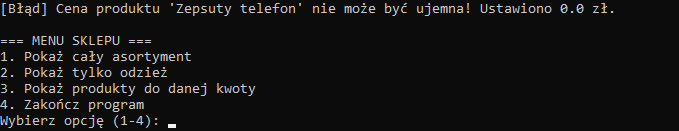
\includegraphics[width=0.8\textwidth]{screen_menu.png}
    \caption{Wyświetlenie komunikatu o błędzie ceny oraz menu głównego programu.}
    \label{fig:program_menu}
\end{figure}

\section{Wyświetlanie całego asortymentu}
Po wpisaniu cyfry 1 i wciśnięciu Enter program pokazuje na ekranie pełną listę produktów znajdujących się w sklepie (Rys. 3.2). Na wydruku widać podział na [Elektronika] oraz [Odzież]. Każdy typ produktu ma swoje własne oznaczenia – elektronika pokazuje czas gwarancji w miesiącach, a odzież rozmiar (np. koszulka NIKE ma rozmiar M). Widać też, że cena zepsutego telefonu została na stałe ustawiona jako $0.00$ zł.

\begin{figure}[H]
    \centering
    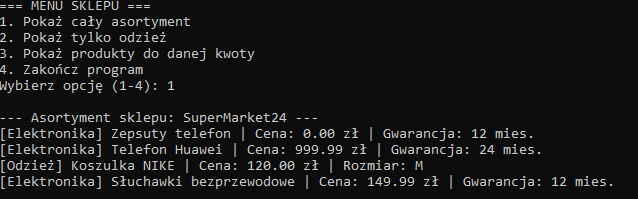
\includegraphics[width=0.8\textwidth]{opcja1.png}
    \caption{Widok konsoli po wybraniu opcji pokazania całego asortymentu.}
    \label{fig:program_asortyment}
\end{figure}

\section{Filtrowanie produktów po kategorii}
Wpisanie w menu cyfry 2 pozwala odfiltrować z całej listy wyłącznie produkty będące odzieżą. Jak widać na Rys. 3.3, po wybraniu tej opcji program pominął telewizor i słuchawki, a na ekranie wypisał tylko koszulkę NIKE wraz z jej rozmiarem i ceną.

\begin{figure}[H]
    \centering
    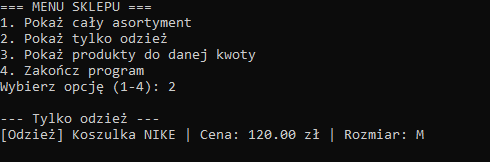
\includegraphics[width=0.8\textwidth]{opcja2.png}
    \caption{Wynik działania filtra wyświetlającego tylko odzież.}
    \label{fig:program_filtrowanie_klas}
\end{figure}

\section{Filtrowanie asortymentu po cenie maksymalnej}
Ostatnia funkcja testowa to opcja numer 3, czyli szukanie produktów do określonej kwoty. Na Rys. 3.4 pokazano sytuację, w której wpisano maksymalną cenę równą $120$ zł. Program automatycznie przeszukał listę i wyświetlił tylko te rzeczy, które mieszczą się w tym limicie: telefon (za $0$ zł) oraz koszulkę NIKE (równe $120$ zł). Droższe przedmioty zostały prawidłowo schowane.

\begin{figure}[H]
    \centering
    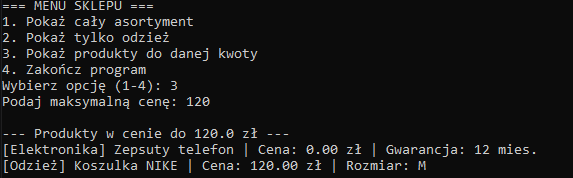
\includegraphics[width=0.8\textwidth]{opcja3.png}
    \caption{Lista produktów odfiltrowana według wpisanej ceny maksymalnej.}
    \label{fig:program_filtrowanie_ceny}
\end{figure}